\documentclass[12pt,a4paper]{report}
\usepackage[utf8]{inputenc}
\usepackage[polish]{babel}
\usepackage[T1]{fontenc}
\usepackage{graphicx}
\usepackage{fancyhdr}
\usepackage{hyperref}
\usepackage{geometry}
\usepackage{booktabs}

\geometry{margin=2.5cm}

\pagestyle{fancy}
\fancyhf{}
\fancyhead[L]{\leftmark}
\fancyhead[R]{\thepage}
\renewcommand{\headrulewidth}{0.4pt}

\title{\textbf{Chińska Republika Ludowa:\\Gospodarka, Kultura i Wpływ Globalny}}
\author{Studentka}
\date{05.12.2025}

\begin{document}

\maketitle

\begin{abstract}
Niniejszy dokument przedstawia kompleksową analizę Chińskiej Republiki Ludowej, koncentrując się na trzech kluczowych aspektach: rozwoju gospodarczym, dziedzictwie kulturowym oraz rosnącej roli na arenie międzynarodowej. Praca omawia transformację Chin z kraju rolniczego w drugą co do wielkości gospodarkę świata, przedstawia bogactwo tradycji kulturowych oraz analizuje współczesne wyzwania i możliwości rozwoju. Dokument został przygotowany w ramach zajęć z tworzenia dokumentów tekstowych w systemie LaTeX.
\end{abstract}

\tableofcontents

\chapter{Wprowadzenie}

Chińska Republika Ludowa stanowi jedno z najważniejszych państw współczesnego świata. Z populacją przekraczającą 1,4 miliarda mieszkańców, Chiny są nie tylko najludniejszym krajem na Ziemi, ale także jedną z najstarszych cywilizacji, której historia sięga ponad 5000 lat wstecz.

Współczesne Chiny przeszły niezwykłą transformację gospodarczą i społeczną, która rozpoczęła się pod koniec lat 70. XX wieku wraz z wprowadzeniem reform rynkowych przez Deng Xiaopinga. Proces ten przekształcił kraj z zacofanej gospodarczo ekonomii centralnie planowanej w globalnego lidera produkcji przemysłowej i drugą największą gospodarkę świata.

Niniejsza praca przedstawia kluczowe aspekty współczesnych Chin, obejmujące:
\begin{itemize}
\item Rozwój gospodarczy i transformację ekonomiczną
\item Bogactwo dziedzictwa kulturowego i tradycji
\item Rolę Chin w globalnej polityce i gospodarce
\item Wyzwania środowiskowe i społeczne
\end{itemize}

\chapter{Gospodarka Chińska}

\section{Transformacja Ekonomiczna}

Od 1978 roku, kiedy to Deng Xiaoping wprowadził politykę reform i otwarcia (gaige kaifang), Chiny doświadczyły bezprecedensowego wzrostu gospodarczego. W ciągu ostatnich czterech dekad PKB Chin wzrosło ponad stokrotnie, wynosząc obecnie ponad 17 bilionów dolarów amerykańskich.

Kluczowe etapy rozwoju gospodarczego można przedstawić następująco:
\begin{enumerate}
\item \textbf{1978-1992:} Wczesne reformy, wprowadzenie Specjalnych Stref Ekonomicznych
\item \textbf{1992-2001:} Przyspieszenie reform rynkowych, przystąpienie do WTO
\item \textbf{2001-2012:} Boom eksportowy i szybki wzrost przemysłu
\item \textbf{2012-obecnie:} Restrukturyzacja gospodarcza i innowacje technologiczne
\end{enumerate}

\section{Handel Międzynarodowy}

Chiny są obecnie największym eksporterem świata oraz drugim co do wielkości importerem. Tabela poniżej przedstawia głównych partnerów handlowych Chin w 2023 roku.

\begin{table}[h]
\centering
\begin{tabular}{@{}lcc@{}}
\toprule
\textbf{Kraj/Region} & \textbf{Eksport (mld USD)} & \textbf{Import (mld USD)} \\ \midrule
Stany Zjednoczone & 500,3 & 164,5 \\
Unia Europejska & 488,9 & 291,2 \\
ASEAN & 518,2 & 441,8 \\
Japonia & 158,7 & 162,1 \\
Korea Południowa & 162,8 & 213,4 \\ \bottomrule
\end{tabular}
\end{table}

Dane w tabeli pokazują, że kraje Azji Południowo-Wschodniej (ASEAN) stanowią obecnie największego partnera handlowego Chin, wyprzedzając tradycyjnie dominujące Stany Zjednoczone i Unię Europejską.

\section{Inicjatywa Pasa i Szlaku}

Rysunek ilustruje zasięg geograficzny inicjatywy Pasa i Szlaku (Belt and Road Initiative, BRI), która została ogłoszona przez prezydenta Xi Jinpinga w 2013 roku. Projekt ten ma na celu rozwój infrastruktury transportowej i gospodarczej łączącej Azję z Europą i Afryką.

\begin{figure}[h]
\centering
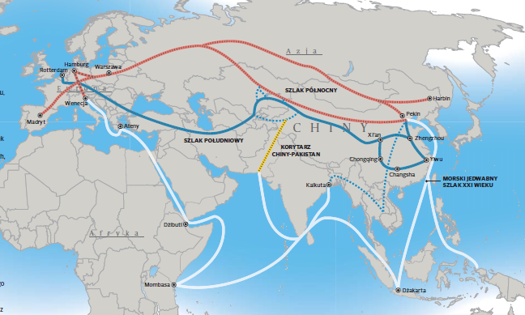
\includegraphics[width=0.9\textwidth]{china_map.png}
\end{figure}
\chapter{Kultura i Tradycja}

\section{Dziedzictwo Historyczne}

Chińska kultura należy do najstarszych nieprzerwanie funkcjonujących cywilizacji na świecie. Fundamentalne wartości konfucjańskie, takie jak szacunek dla autorytetu, harmonia społeczna i lojalność rodzinna, nadal odgrywają istotną rolę we współczesnym społeczeństwie chińskim.

\section{Język i Pismo}

Język chiński (Hanyu) wykorzystuje logograficzny system pisma liczący ponad 50 000 znaków, choć do codziennej komunikacji wystarczy znajomość około 3000-4000 znaków. Współczesny język mandaryński (Putonghua) jest oficjalnym językiem kraju i jednym z sześciu oficjalnych języków Organizacji Narodów Zjednoczonych.

\section{Sztuka i Architektura}

Chińska sztuka tradycyjna obejmuje szeroki zakres dziedzin:
\begin{itemize}
\item Malarstwo tuszem i kaligrafię
\item Ceramikę i porcelanę (słynna porcelana z Jingdezhen)
\item Sztukę ogrodową i architekturę krajobrazową
\item Operę Pekińską (Jingju)
\item Tradycyjną muzykę instrumentalną
\end{itemize}

\chapter{Rola Globalna i Wyzwania}

\section{Pozycja Międzynarodowa}

Chiny są stałym członkiem Rady Bezpieczeństwa ONZ i odgrywają kluczową rolę w organizacjach międzynarodowych takich jak G20, BRICS czy Szanghajska Organizacja Współpracy. Rosnące znaczenie gospodarcze przekłada się na wzrost wpływów politycznych i dyplomatycznych.

\section{Wyzwania Środowiskowe}

Szybka industrializacja przyniosła poważne problemy ekologiczne. Chiny są obecnie największym emitentem dwutlenku węgla na świecie, choć jednocześnie prowadzą ambitną politykę ochrony środowiska, deklarując osiągnięcie neutralności węglowej do 2060 roku. Kraj jest światowym liderem w produkcji i instalacji odnawialnych źródeł energii, szczególnie energii słonecznej i wiatrowej.

\chapter{Wnioski}

\section{Uzasadnienie Wyboru Klasy Report}

Do przygotowania niniejszego dokumentu wybrano klasę \texttt{report} z następujących powodów:
\begin{enumerate}
\item Dokument ma charakter akademicki i zawiera kilka rozdziałów tematycznych.
\item Klasa \texttt{report} umożliwia łatwe zarządzanie strukturą wielorozdziałową.
\item Dostępne są wbudowane mechanizmy do tworzenia strony tytułowej i abstraktu.
\item Struktura dokumentu nie wymaga podziału na części (\texttt{part}), które są bardziej charakterystyczne dla klasy \texttt{book}.
\item Dla dokumentów o podobnej objętości klasa \texttt{report} jest bardziej odpowiednia niż \texttt{article}.
\end{enumerate}

Klasa \texttt{book} byłaby bardziej uzasadniona dla znacznie obszerniejszych prac, które wymagają podziału na części oraz druku dwustronnego z rozróżnieniem stron lewych i prawych.

\section{Podsumowanie}

Chińska Republika Ludowa stanowi fascynujący przykład kraju, który w ciągu zaledwie kilku dekad przeszedł drogę od izolacji do pozycji globalnego mocarstwa gospodarczego. Bogata historia i kultura łączą się z nowoczesnością i technologicznym rozwojem, tworząc unikalny model rozwoju społeczno-gospodarczego.

Przyszłość Chin będzie miała kluczowe znaczenie dla całego świata, szczególnie w kontekście wyzwań związanych ze zmianami klimatu, równowagą geopolityczną i rozwojem technologicznym.

\section{Repozytorium}

Źródła dokumentu dostępne są w repozytorium git pod adresem: \\
\url{https://github.com/MajaHarazna/LaTeX---tworzenie-dokument-w-tekstowych}

\begin{thebibliography}{9}

\bibitem{wiki_china}
Wikipedia contributors. (2024). \textit{China}.
Wikipedia, The Free Encyclopedia. \\
\url{https://en.wikipedia.org/wiki/China}

\bibitem{worldbank_china}
The World Bank. (2024). \textit{China Overview}.
World Bank Group. \\
\url{https://www.worldbank.org/en/country/china/overview}

\bibitem{imf_data}
International Monetary Fund. (2024). \textit{World Economic Outlook Database}.
IMF. \\
\url{https://www.imf.org/en/Publications/WEO}

\bibitem{china_customs}
General Administration of Customs of China. (2024). \textit{Statistics}.\\
\url{http://english.customs.gov.cn/}

\bibitem{confucius_inst}
Confucius Institute. (2024). \textit{Chinese Culture and Philosophy}.\\
\url{https://www.confuciusinstitute.ac.uk/}

\bibitem{un_china}
United Nations. (2024). \textit{China and the United Nations}.\\
\url{https://www.un.org/en/}

\bibitem{bri_map}
Bankier.pl. (2019). \textit{Pas i Szlak - chińska pułapka kredytowa? Analiza}.\\
\url{https://www.bankier.pl/wiadomosc/Pas-i-Szlak-chinska-pulapka-kredytowa-Analiza-7576219.html}\\
Źródło mapy inicjatywy Pasa i Szlaku.

\end{thebibliography}


\end{document}
